\documentclass [xcolor=svgnames] {beamer} 
\usepackage[utf8]{inputenc}
\usepackage{xcolor}
\usepackage{booktabs, comment} 
\usepackage{pgfpages}
\usepackage{csquotes}
\usepackage{amsmath}
\usepackage{tikz}
\usepackage{caption}
\usepackage{subcaption}
\usetheme{Madrid}

% COLORS 
\definecolor{mqred}{RGB}{166, 25, 46}
\definecolor{mqdeepred}{RGB}{118, 35, 47}
\definecolor{mqgray}{RGB}{55, 58, 54}
\definecolor{mqlightgray}{RGB}{237, 235, 229}
\definecolor{mqmagenta}{RGB}{198, 0, 126}
\usecolortheme[named=mqred]{structure}
\setbeamercolor{title in head/foot}{bg=mqlightgray, fg=mqgray}
\setbeamercolor{author in head/foot}{bg=mqdeepred}
\setbeamercolor{page number in head/foot}{bg=mqdeepred, fg=mqlightgray}

% FOOTNOTE ARRANGEMENTS

\makeatletter
\setbeamertemplate{footline}{
	\leavevmode%
	\hbox{%
		\begin{beamercolorbox}[wd=.5\paperwidth,ht=2.25ex,dp=1ex,center]{author in head/foot}%
			\usebeamerfont{author in head/foot}\insertshortauthor\expandafter\ifblank\expandafter{\beamer@shortinstitute}{}{~~(\insertshortinstitute)}
		\end{beamercolorbox}%
		\begin{beamercolorbox}[wd=.4\paperwidth,ht=2.25ex,dp=1ex,center]{title in head/foot}%
			\usebeamerfont{title in head/foot}\insertshorttitle
		\end{beamercolorbox}%
		\begin{beamercolorbox}[wd=.1\paperwidth,ht=2.25ex,dp=1ex,center]{page number in head/foot}%
			\usebeamerfont{page number in head/foot}\insertframenumber{} / \inserttotalframenumber 
	\end{beamercolorbox}}%
	\vskip0pt%
}
\makeatother
\beamertemplatenavigationsymbolsempty


% TITLE, AUTHORS, INSTITUTE, DATE

\title[Short Title]{Caratterizzazione di un rivelatore gamma 4$\pi$ per lo studio della reazione 14N(p,$\gamma$)15O \\ \textit{Relatrice: Francesca Cavanna}}
\author[P. Pusterla]{Paolo Pusterla}
\institute[UniTo]{Università degli Studi di Torino}
\date{Novembre 2024}

% LOGO
\titlegraphic{
\includegraphics[height=2.5cm]{img/logo.png}} % Change the logo path as needed

%add table of contents before each section
\AtBeginSection[]
{
	\begin{frame}
		\frametitle{Table of Contents}
		\tableofcontents[currentsection]
	\end{frame}
}

\begin{document}
	
	\begin{frame}
		\titlepage
	\end{frame}
	
	\begin{frame}{Outline}
		\tableofcontents
	\end{frame}
	
	% Section and Frame examples
	\section{Introduzione}
	\begin{frame}{L'esperimento}
		\begin{itemize}
			\item<1-> L'esperimento LUNA (Laboratory for Underground Nuclear Astrophysics) ricrea i processi nucleari che sono avvenuti durante la nucleosintesi primordiale e che avvengono tutt'ora nelle stelle.
			\item<2-> Essendo processi molto rari, un laboratorio sulla superficie terrestre non è adatto per le misure sperimentali di questi, poiché i raggi cosmici maschererebbero il segnale debole atteso.
		\end{itemize}
	\end{frame}
	
	
	\begin{frame}{Proposta dell'esperimento}
		\begin{itemize}
			\item<1-> I neutrini solari giocano un ruolo fondamentale nella determinazione della composizione del Sole.
			\item<2-> Sono prodotti nel ciclo CNO del Sole.
			\item<3-> In particolare, la sezione d'urto della reazione $^{14}$N(p, $\gamma$)$^{15}$O è la fonte di errore principale sulle stime del flusso di neutrini.
		\end{itemize}
	\end{frame}
		
	\begin{frame}{Il ciclo CNO}
		\begin{figure}[H]
			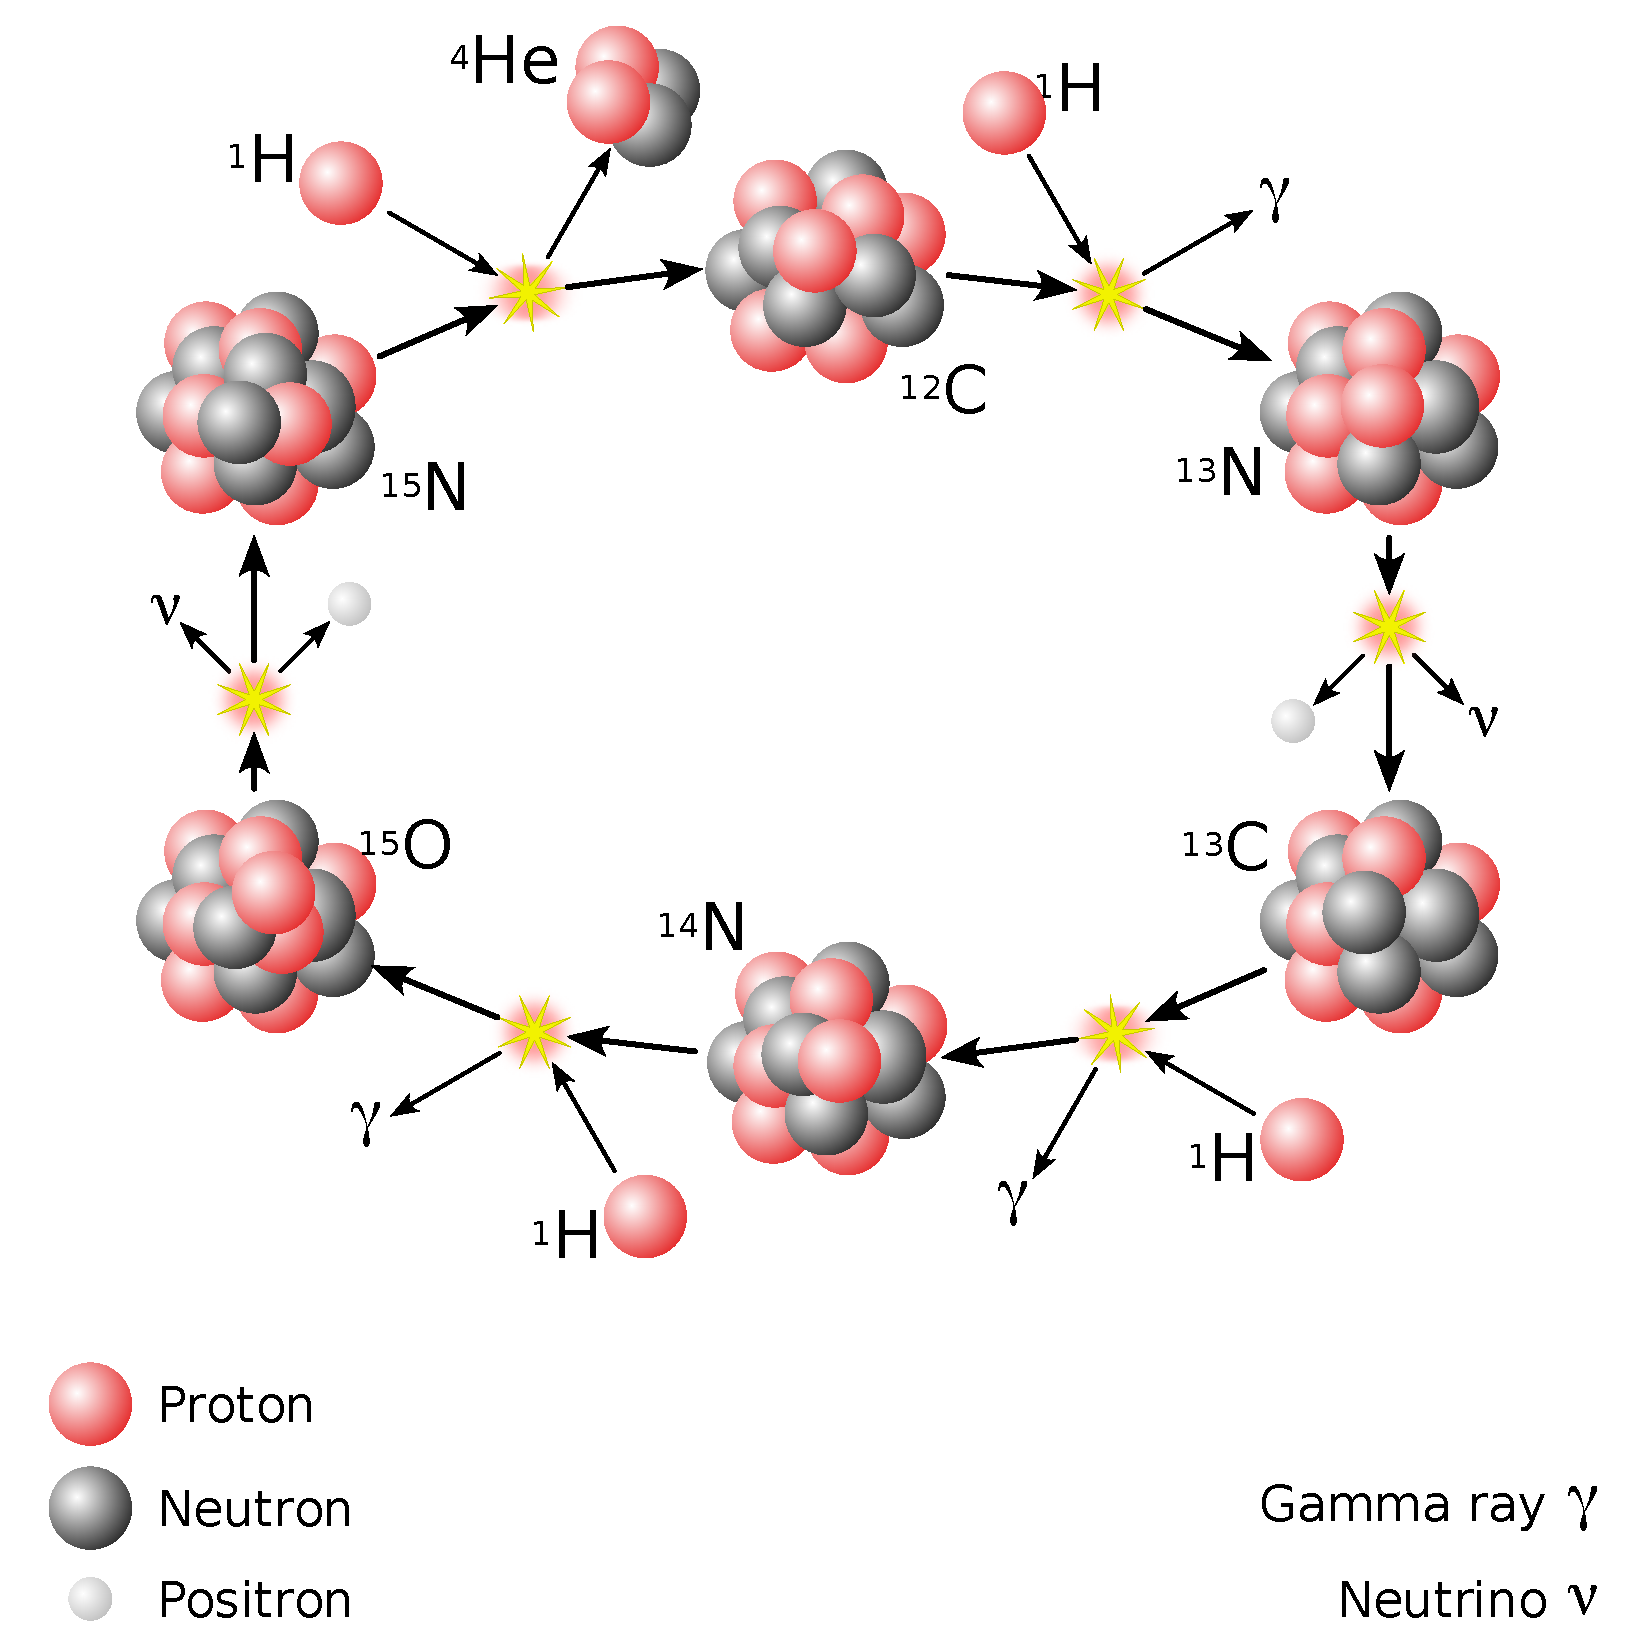
\includegraphics[width=0.5\textwidth]{img/CNO_Cycle.pdf}
			\caption{Ciclo Carbonio-Azoto-Ossigeno}
		\end{figure}
	\end{frame}
	
	\begin{frame}{Proposta dell'esperimento}
		\begin{itemize}
			\item<1-> A energie solari (15-50 keV) la sezione d'urto è troppo piccola per essere misurata direttamente.
			\item<2-> Le stime odierne sono quindi estrapolazioni da energie più alte.
			\item<3-> Il progetto ha come obiettivo determinare la sezione d'urto ad energie 50-370 keV.
		\end{itemize}
	\end{frame}
	
%\begin{frame}{Sfide sperimentali della misura diretta}
%	\begin{itemize}
%		\item La \emph{sezione d'urto} di una reazione nucleare è una grandezza utilizzata per descrivere la probabilità che la reazione avvenga.
%		\item La si può calcolare sperimentalmente come:
%	\end{itemize}
%	
%	\begin{equation}
%		\sigma = 
%		\dfrac{
%			\only<1>{\tikz[baseline]{\node[anchor=base,draw,rectangle,red,thick,inner sep=2pt] (num) {$N_{reaz}/\Delta t$};}} % First slide
%			\only<2>{N_{reaz}/\Delta t} % Normal text for slide 2 and 3
%		}{
%			\only<2>{\tikz[baseline]{\node[anchor=base,draw,rectangle,red,thick,inner sep=2pt] (proj) {$N_{proj} / \Delta t$};}} % Second slide
%			\only<1-2>{N_{proj} / \Delta t} % Normal text for slides 1 and 2
%			\times
%			\only<3>{\tikz[baseline]{\node[anchor=base,draw,rectangle,red,thick,inner sep=2pt] (bers) {$N_{bers} / A$};}} % Third slide
%			\only<1-2>{N_{bers} / A} % Normal text for slides 1 and 2
%		}
%	\end{equation}
%	
%	% Slide 1 explanation for numerator
%	\only<1>{
%		\begin{tikzpicture}[overlay]
%			\draw[->, red, thick] (num.east) -- ++(1,0) node[right] {Numero di reazione per unità di tempo};
%		\end{tikzpicture}
%	}
%	
%	% Slide 2 explanation for N_proj / Delta t
%	\only<2>{
%		\begin{tikzpicture}[overlay]
%			\draw[->, red, thick] (proj.east) -- ++(1,0) node[right] {Numero di proiettili per unità di tempo};
%		\end{tikzpicture}
%	}
%	
%	% Slide 3 explanation for N_bers / A
%	\only<3>{
%		\begin{tikzpicture}[overlay]
%			\draw[->, red, thick] (bers.east) -- ++(1,0) node[right] {Numero di bersagli per unità di area};
%		\end{tikzpicture}
%	}
%	
%\end{frame}


\begin{frame}{Sfide sperimentali della misura diretta}
	\begin{itemize}
		\item<1-> La \emph{sezione d'urto} di una reazione nucleare è una grandezza utilizzata per descrivere la probabilità che la reazione avvenga.
		\item<2-> La si può calcolare sperimentalmente come:
		\begin{equation}
			\sigma = \dfrac{N_{reaz}/\Delta t}{N_{proj}/\Delta t \times N_{bers}/A \times \varepsilon}
		\end{equation}
	\item<3-> $N_{reaz}/\Delta t$ è il numero di reazioni per unità di tempo;
	\item<4-> $N_{proj}/\Delta t \approx 10^{14}$ pps per intensità tipiche di un fascio stabile
	\item<5-> $N_{bers}/A \approx 10^{19}$ atomi/cm per un tipico bersaglio allo stato solido
	\item<6-> $\sigma \approx 10^{-12}$ barn, spesso è anche più piccola
	\item<7-> $\varepsilon \approx 1 \div 10 \%$ per i raggi gamma
	\end{itemize}
\end{frame}
\begin{frame}{Reaction rate}
	\begin{itemize}
		\item<1-> Il \emph{reaction rate} vale quindi appena $1\div 10$ conteggi al giorno
		\item<2-> Basta pochissimo rumore per nascondere i segnali che rivelano le reazioni
		\item<3-> La soluzione è cercare di minimizzare il rumore di fondo 
	\end{itemize}
\end{frame}

	\begin{frame}{Località}
		\begin{columns}
			\begin{column}{0.5\textwidth}
				\begin{itemize}
					\item<1-> I Laboratori Nazionali del Gran Sasso, situati nella frazione di Assergi, sono schermati dai 1400 m di roccia del Monte Aquila.
					\item<2-> Ciò fa sì che il fondo di raggi cosmici sia fortemente soppresso
					\item<3-> Qui è collocato l'acceleratore LUNA2 a 400 kV, in attività dal 2001, che permette di concentrare fasci ionici molto intensi e stabili.
				\end{itemize}
			\end{column}
			\begin{column}{0.5\textwidth}
				\centering
				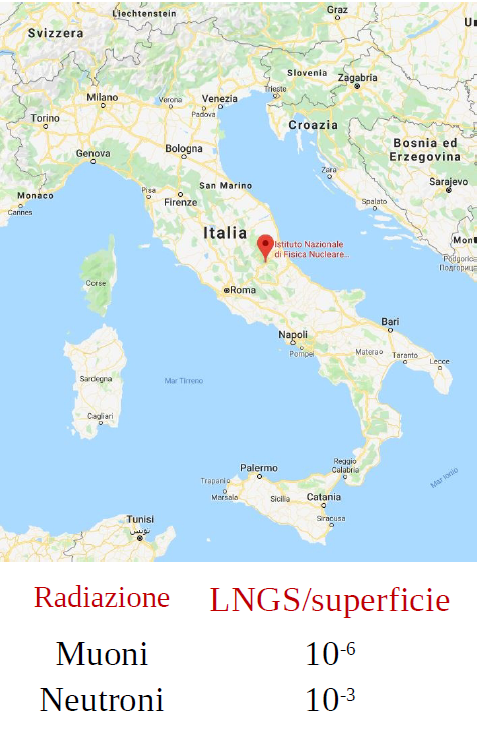
\includegraphics[width=0.8\textwidth]{img/location.png}
				\captionof{figure}{LNGS, Assergi, AQ.}
			\end{column}
		\end{columns}
	\end{frame}
	
	\begin{frame}{L'acceleratore}
		\centering
		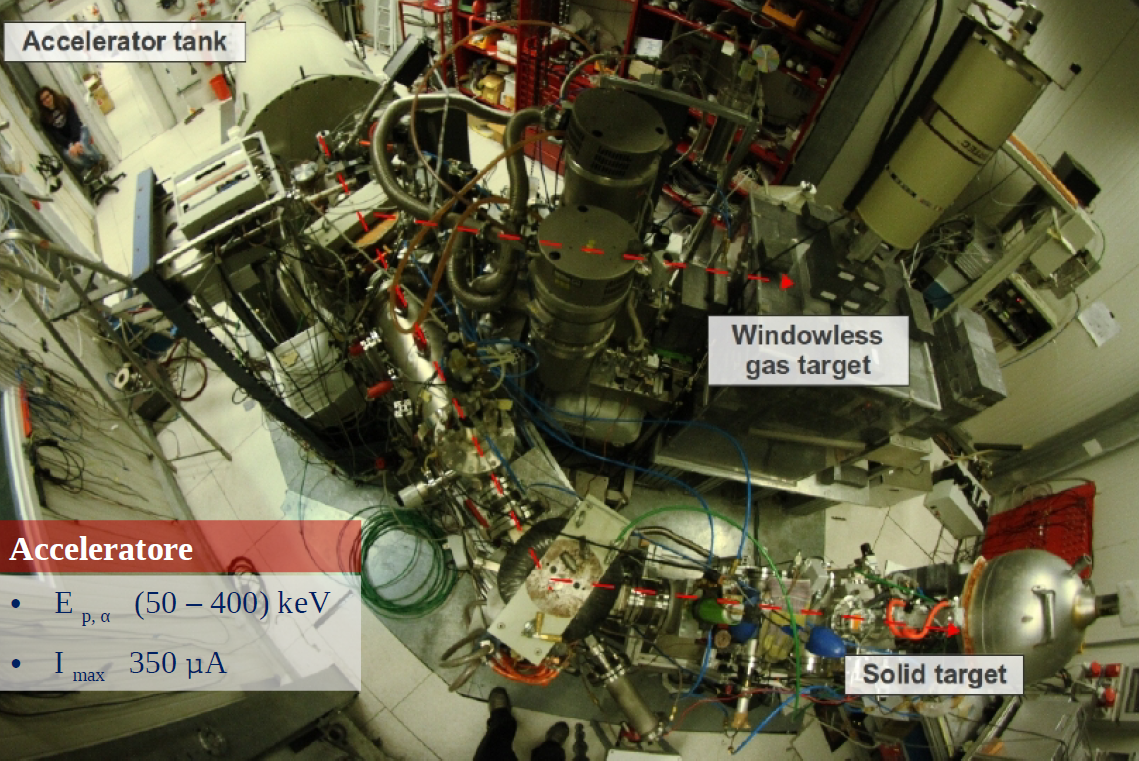
\includegraphics[width=0.9\textwidth]{img/LUNA2.png}
		\captionof{figure}{L'acceleratore LUNA2 a 400 kV.}
	\end{frame}
	
	\begin{frame}{Fondo}
		\centering
		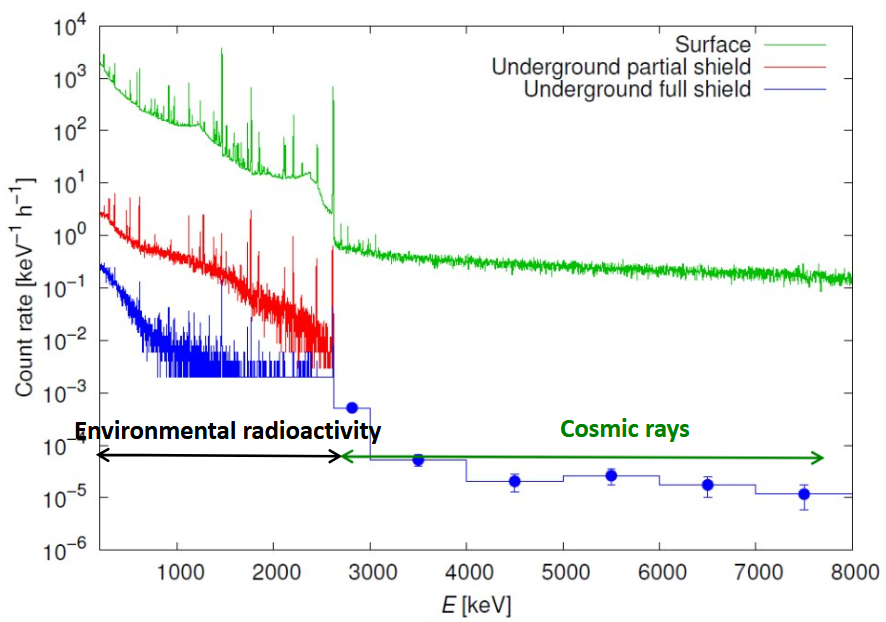
\includegraphics[width=0.7\textwidth]{img/noise.png}
		\captionof{figure}{Grafico riportante il rumore di fondo in superficie, sotto una schermatura parziale sottoterra e sotto una schermatura totale sottoterra.}
	\end{frame}
	
	\section{Obiettivi della tesi}
	\begin{frame}{Obiettivi della tesi}
		\begin{itemize}
			\item<1-> L'obiettivo della tesi è quello di caratterizzare in efficienza lo scintillatore $4\pi$ utilizzato per la rivelazione di raggi $\gamma$ nella riproduzione della reazione $^{14}$N(p,$\gamma$)$^{15}$O. 
			\item<2-> Nell'esperimento si proietta un intenso fascio di protoni su bersagli solidi di TiN (nitruro di titanio).  
		\end{itemize}
	\end{frame}

	\section{Il rivelatore}
	\begin{frame}{Il rivelatore $4\pi$}
		\begin{columns}
			\begin{column}{0.45\textwidth}
				\begin{itemize}
					\item La radiazione gamma emessa dalla reazione è rivelata da uno scintillatore.
					\item Si tratta di un rivelatore in germanato di bismuto (Bi$_{4}$Ge$_{3}$O$_{12}$, detto BGO), coprente il 95\% dell'angolo solido totale attorno al bersaglio.
				\end{itemize}
			\end{column}
			\begin{column}{0.45\textwidth}
				\centering
				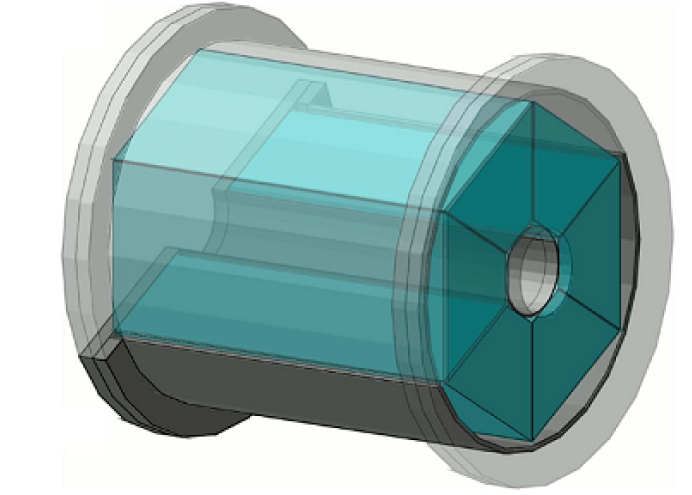
\includegraphics[width=\textwidth]{img/bgo_3d.png}
				\captionof{figure}{Rappresentazione 3D del rivelatore BGO.}
			\end{column}
		\end{columns}
		
	\end{frame}

\begin{frame}{Il rivelatore $4\pi$}
	\begin{columns}
		\begin{column}{0.45\textwidth}
			\begin{itemize}
				\item Il cristallo, a simmetria cilindrica, è otticamente separato in 6 spicchi uguali.
				\item I fotoni di scintillazione di ciascuno dei 6 segmenti sono rivelati da due fotomoltiplicatori.
			\end{itemize}
		\end{column}
		\begin{column}{0.45\textwidth}
			\centering
			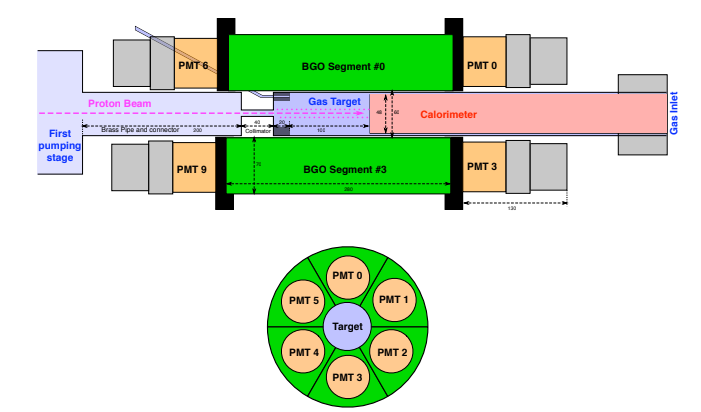
\includegraphics[width=\textwidth]{img/BGO.png}
			\captionof{figure}{Rappresentazione schematica del rivelatore BGO. In alto una sezione sagittale, in basso una sezione trasversale.}
		\end{column}
	\end{columns}
\end{frame}


\begin{frame}{Efficienza}
	\begin{itemize}
		\item L'efficienza di uno scintillatore è il rapporto tra il numero di conteggi prodotti da esso e il numero di conteggi prodotti dalla sorgente:
		
		\begin{equation}
			\varepsilon = \dfrac{N_{\gamma}}{N_{int}}
		\end{equation}
		
		\item Si tratta pertanto di quanti fotoni lo strumento "vede" rispetto al totale
		\item Invertendo l'equazione possiamo ricavare $N_{int}$, per poi trovare la sezione d'urto
	\end{itemize}
\end{frame}

\begin{frame}{Efficienza}
	\begin{itemize}
		\item Nel caso dei nostri istogrammi, composti da un picco gaussiano centrato su un'energia caratteristica e un fondo di \emph{bremsstrahlung}, l'efficienza si può stimare nel modo seguente:
		
		\begin{equation}
			\varepsilon = \dfrac{N_{cont.}}{A(t*) \Delta t}
		\end{equation}
	
		dove $N_{cont.}$ è il numero di conteggi del picco gaussiano sottraendone il fondo, $A(t*)$ è l'attività calcolata al momento della misura, $\Delta t$ è il tempo "vivo" dello strumento.
	\end{itemize}
\end{frame}

\begin{frame}{Tempo vivo/morto}
	\begin{itemize}
		\item Ogni strumento è elettronicamente vincolato a processare il segnale in ingresso
		\item Questo può richiedere fino a ns
		\item Un fotone in arrivo durante questo intervallo di tempo non può essere quindi rilevato
		\item Alla fine della misura verrano osservati meno fotoni di quelli effettivamente giunti allo strumento, perché quest'ultimo è attivo solo per una parte di tempo rispetto al totale della misura.
		\item L'intervallo in cui lo strumento è attivo e pronto a ricevere nuovi segnali è il \emph{tempo vivo}.
	\end{itemize}
\end{frame}

\section{Caratterizzazione}
\begin{frame}{Caratterizzazione in energia}
	\begin{itemize}
		\item La caratterizzazione in energia è effettuata utilizzando due sorgenti radioattive: $^{60}$Co e $^{137}$Cs.
	\end{itemize}
\end{frame}

\begin{frame}{$^{60}$Co}


			\begin{itemize}
				\item<1-> Il $^{60}$Co decade tramite decadimento $\beta^{-}$ (99.75\%) in $^{60}$Ni ed emette due raggi gamma di energie 1.17 MeV e 1.33 MeV.
				\item<2-> Ha il vantaggio di emettere raggi gamma ad alta intensità con un'emivita relativamente lunga di 5.27 anni. 
				\item<3-> Trova applicazione nella radioterapia del cancro.
			\end{itemize}

		\centering
		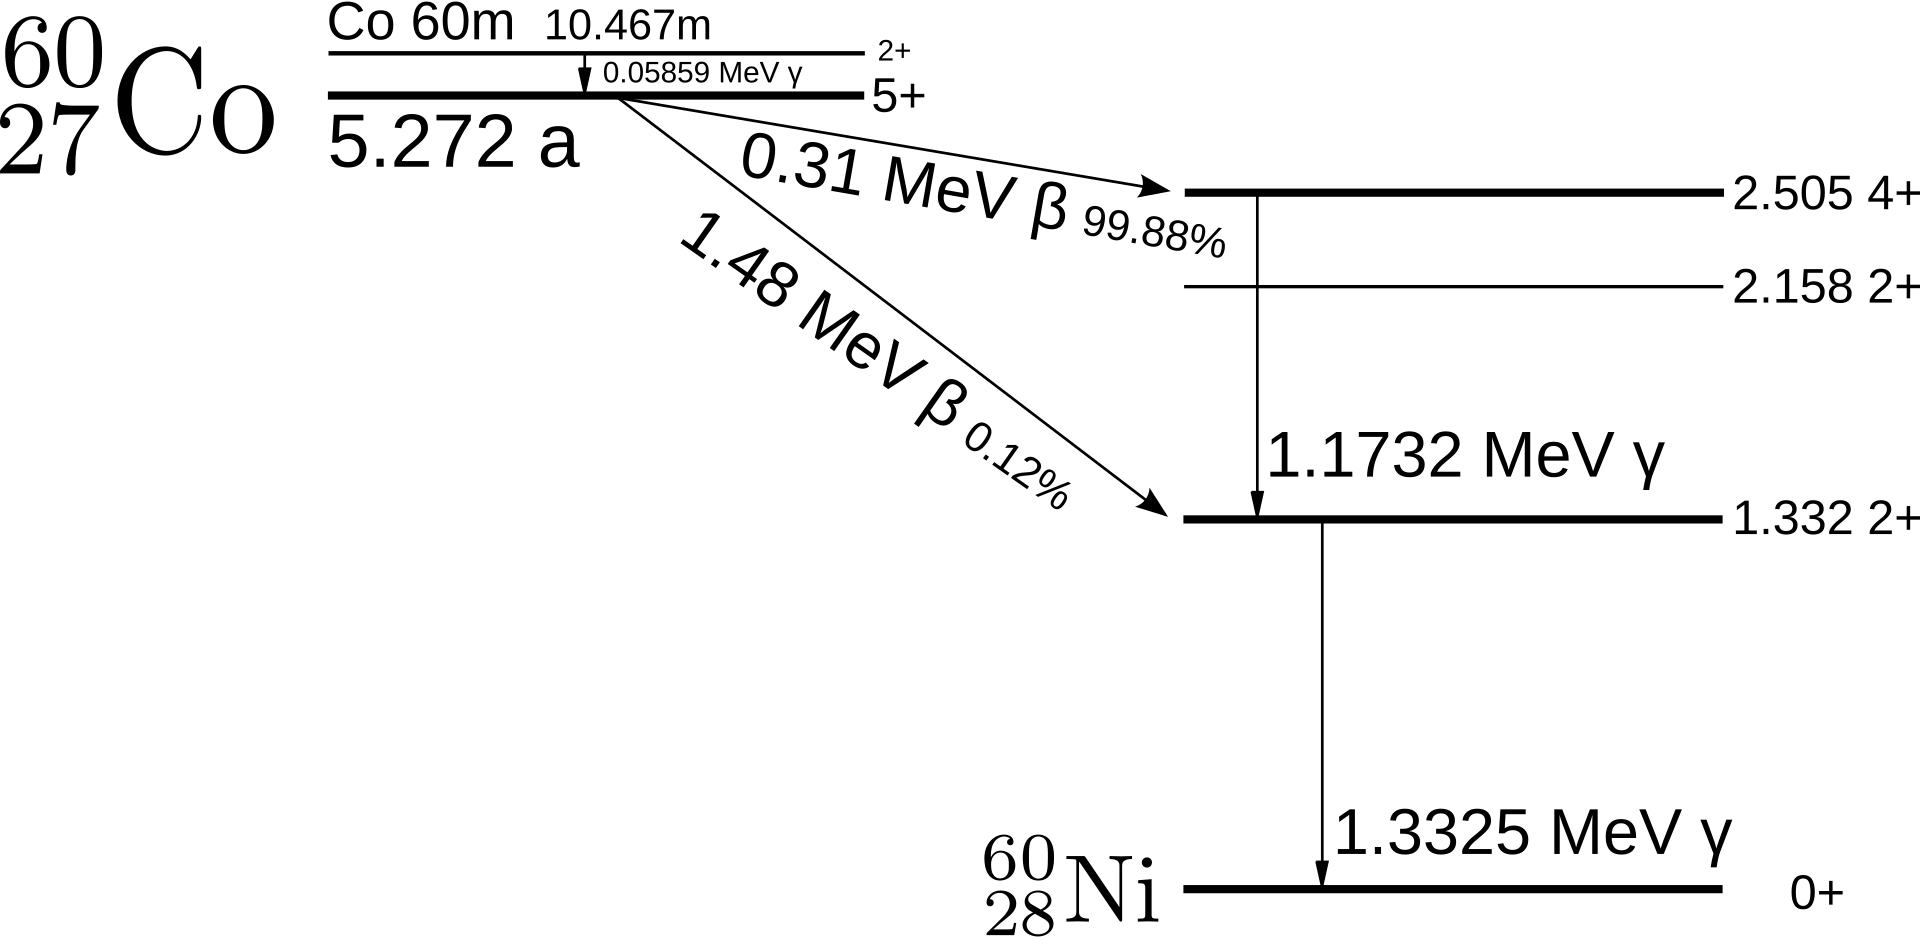
\includegraphics[width=0.5\textwidth]{img/Cobalt-60m-decay.png}
		\captionof{figure}{Schema di decadimento del $^{137}$Cs.}

\end{frame}

\begin{frame}{$^{137}$Cs}
	\begin{itemize}
		\item<1-> Il $^{137}$Cs decade sempre tramite decadimento $\beta^{-}$.
		\item<2-> Il 94.6\% dei decadimenti hanno come prodotto uno stato metastabile del $^{137}$Ba. 
		\item<3-> Questo stato eccitato emette l'85\% delle volte raggi gamma di 661.7 keV decadendo nello stato fondamentale del $^{137}$Ba (tutti i raggi gamma provenienti dal $^{137}$Cs sono prodotti così).
	\end{itemize}
		\centering
		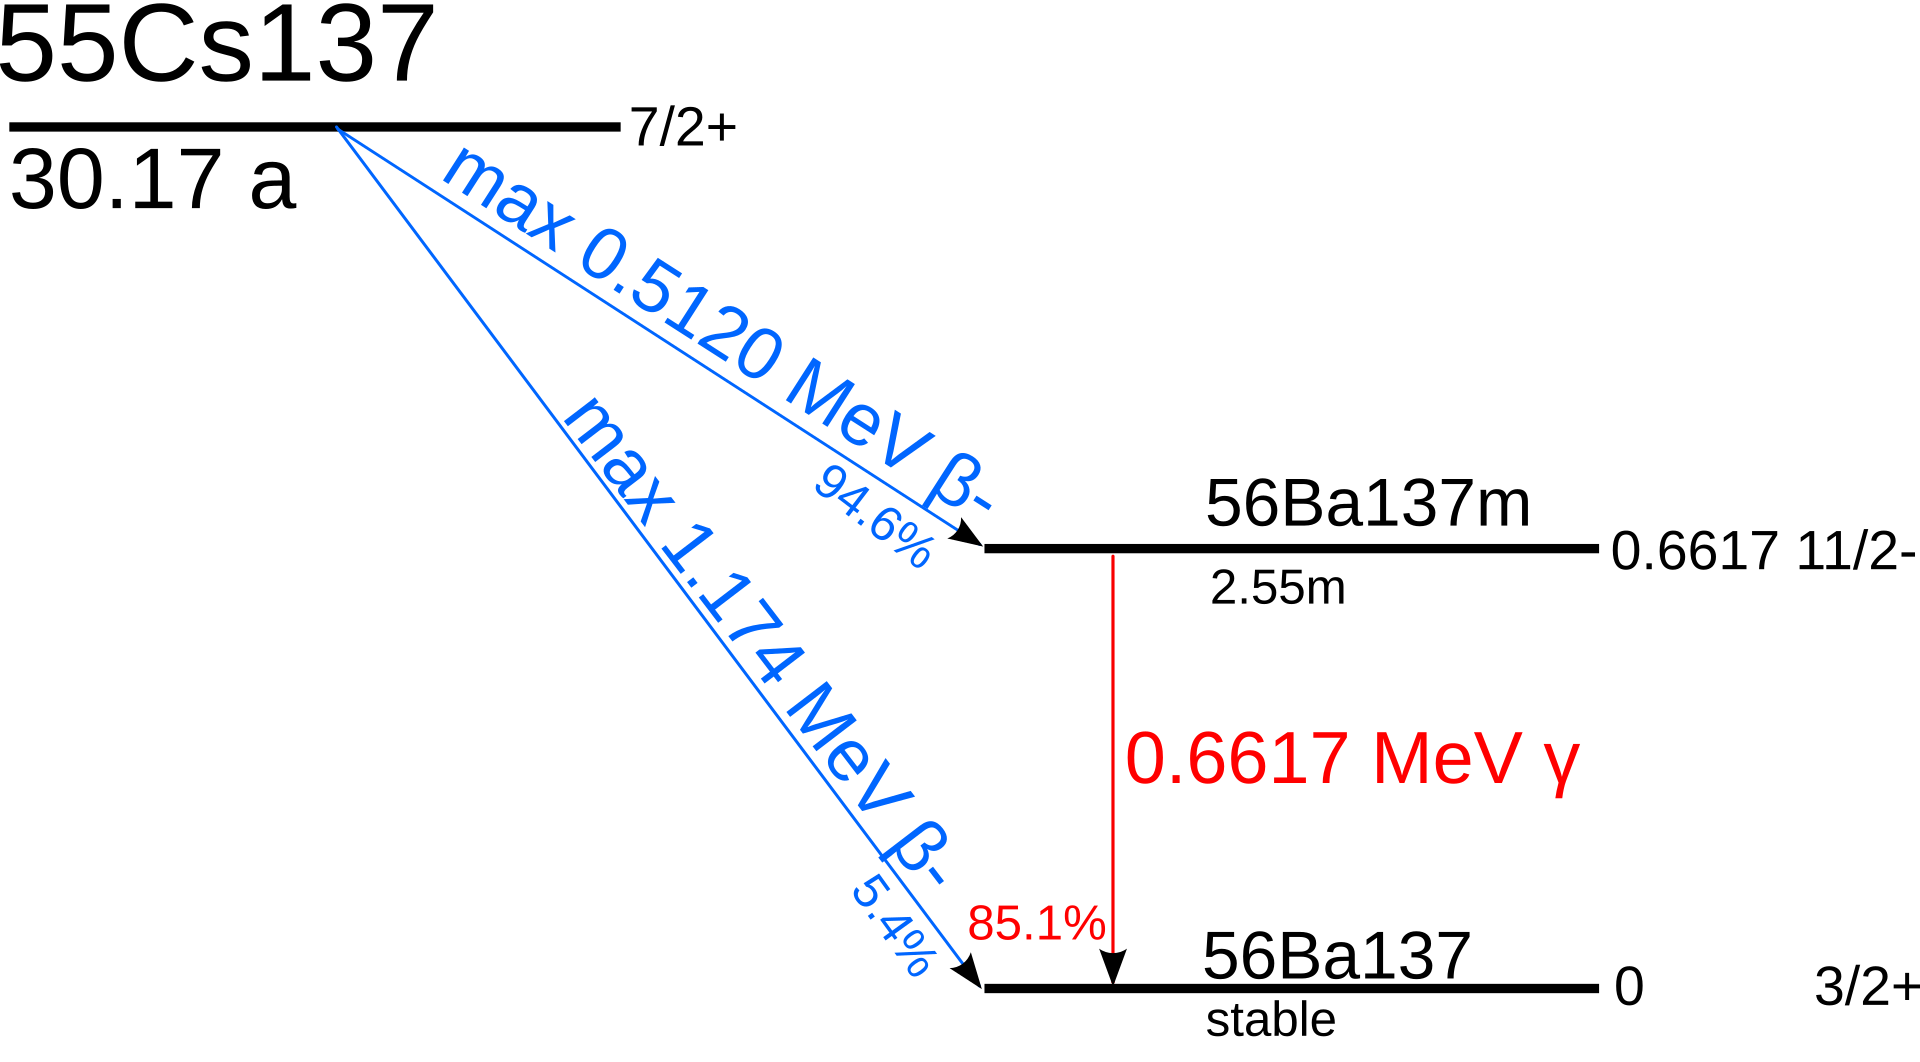
\includegraphics[width=0.5\textwidth]{img/Cs-137-decay.png}
		\captionof{figure}{Schema di decadimento del $^{137}$Cs.}
\end{frame}

\begin{frame}{Struttura dei dati}
	\begin{itemize}
		\item I dati ricavati sono contenuti in file \texttt{.root}
		\item Ogni file \texttt{.root} contiene 8 istogrammi, con indici da 0 a 7, di conteggi
		\item L'istogramma 0 contiene il pulser, utilizzato per calcolare il tempo vivo dello scintillatore
		\item Gli istogrammi da 1 a 6 sono i singoli spicchi del BGO
		%\item L'istogramma 7 è
	\end{itemize}
\end{frame}

\begin{frame}{Istogrammi}
	\begin{figure}
		\centering
		\begin{minipage}{0.45\textwidth}
			\centering
			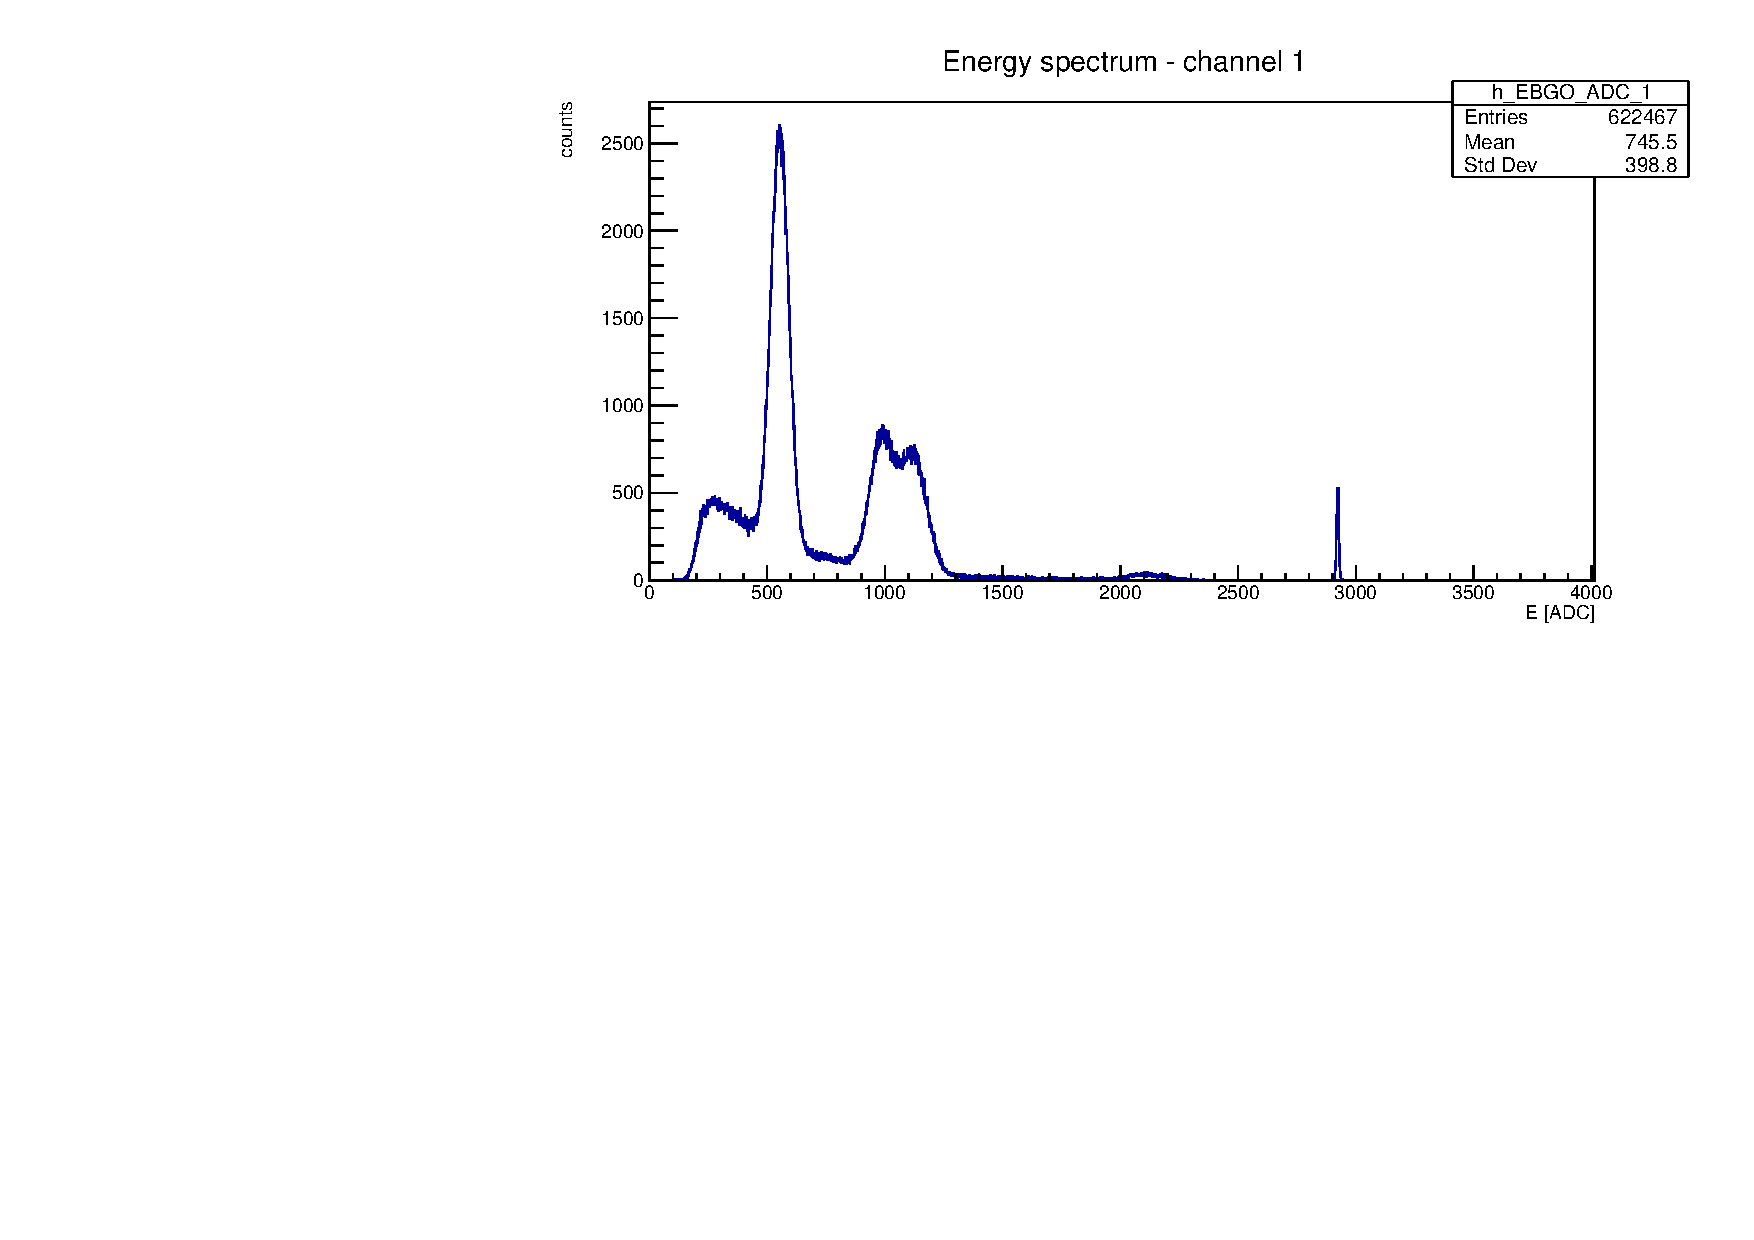
\includegraphics[width=\linewidth]{img/ex1775.pdf} % Replace with your image path
		\end{minipage}
		\hfill
		\begin{minipage}{0.45\textwidth}
			\centering
			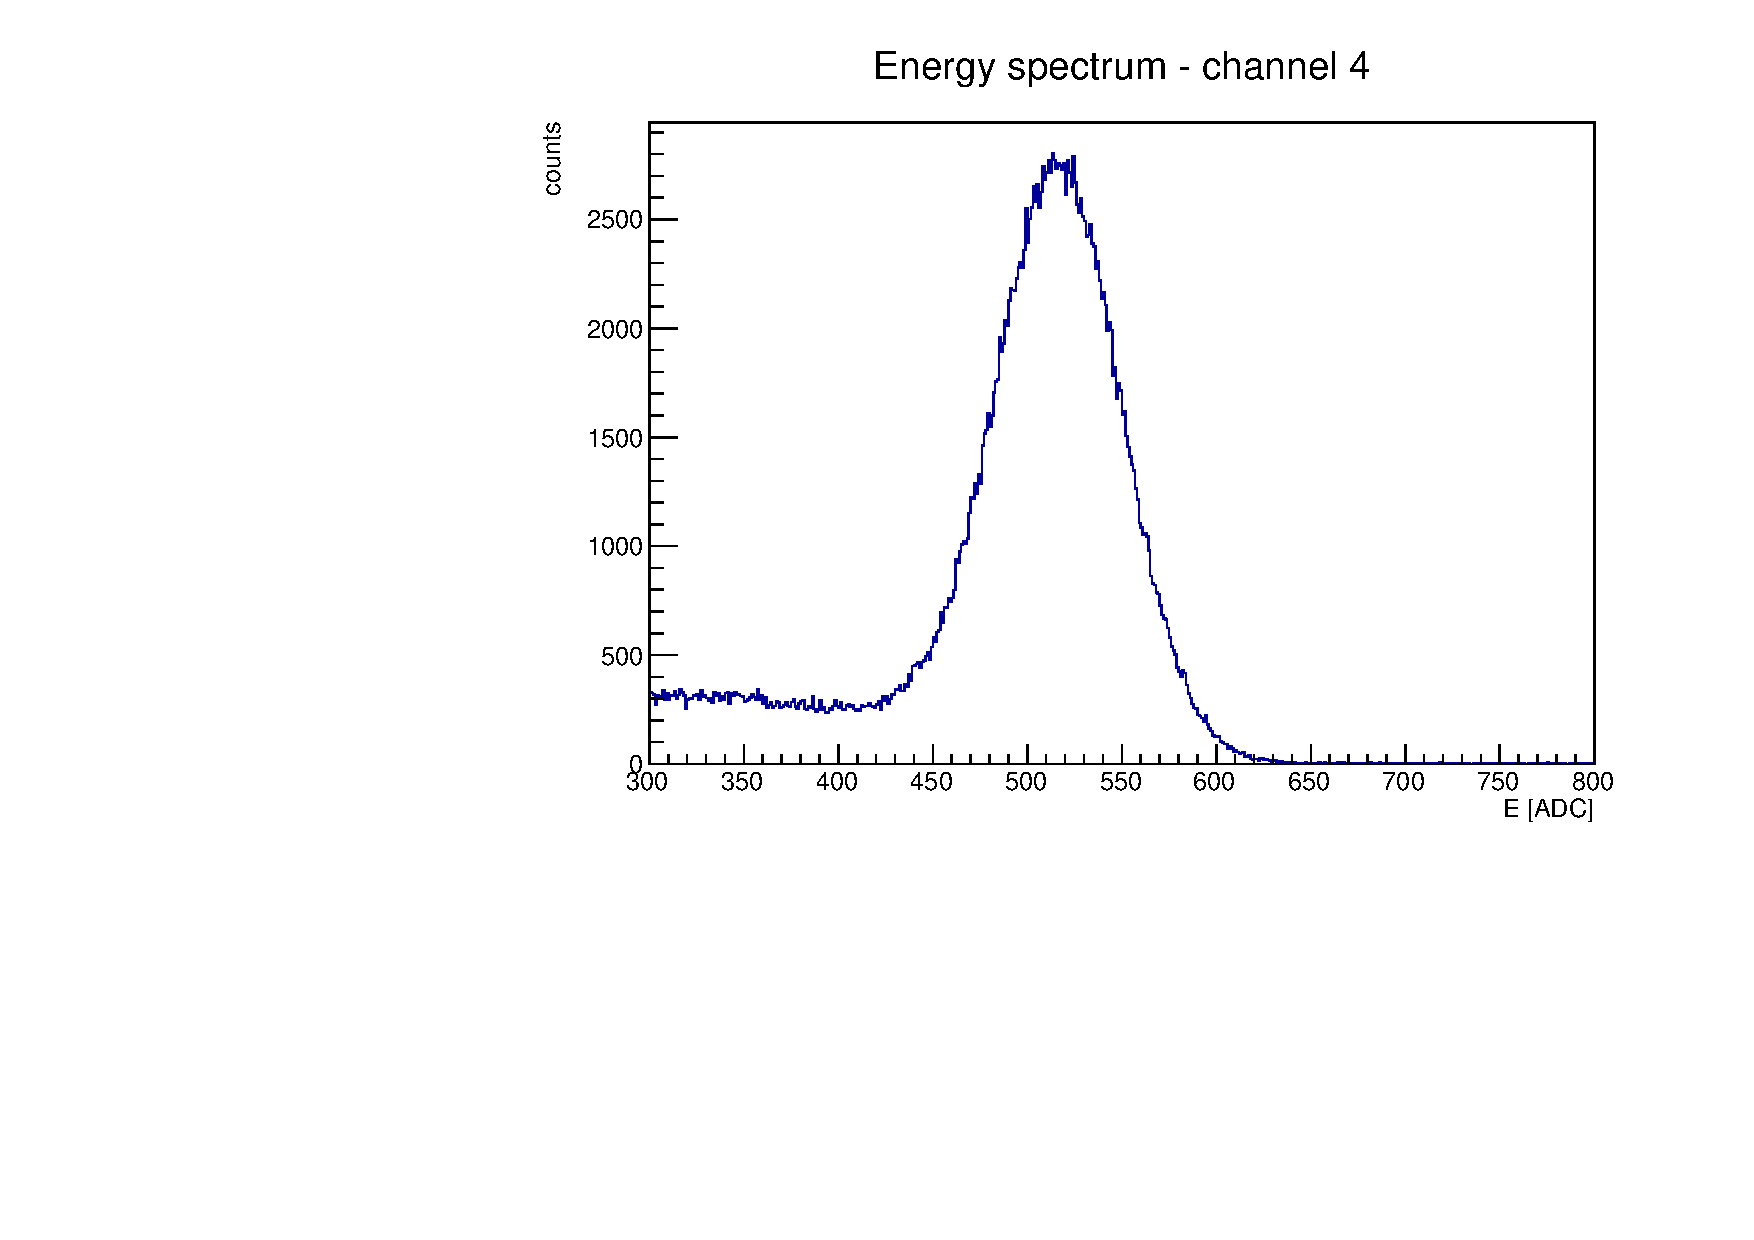
\includegraphics[width=\linewidth]{img/ex1776.pdf} % Replace with your image path
		\end{minipage}
		
		\vspace{0.4cm} % Adjust vertical space between rows
		
		\begin{minipage}{0.45\textwidth}
			\centering
			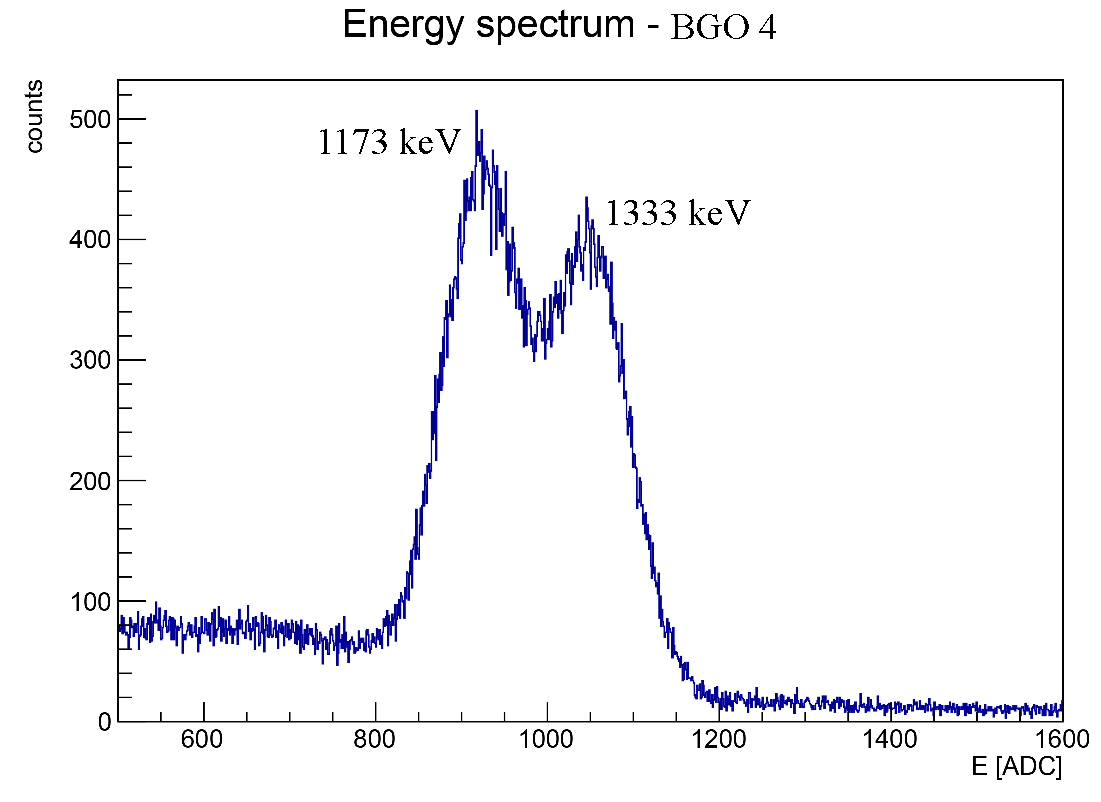
\includegraphics[width=\linewidth]{img/ex1777.pdf} % Replace with your image path
		\end{minipage}
		\hfill
		\begin{minipage}{0.45\textwidth}
			\centering
			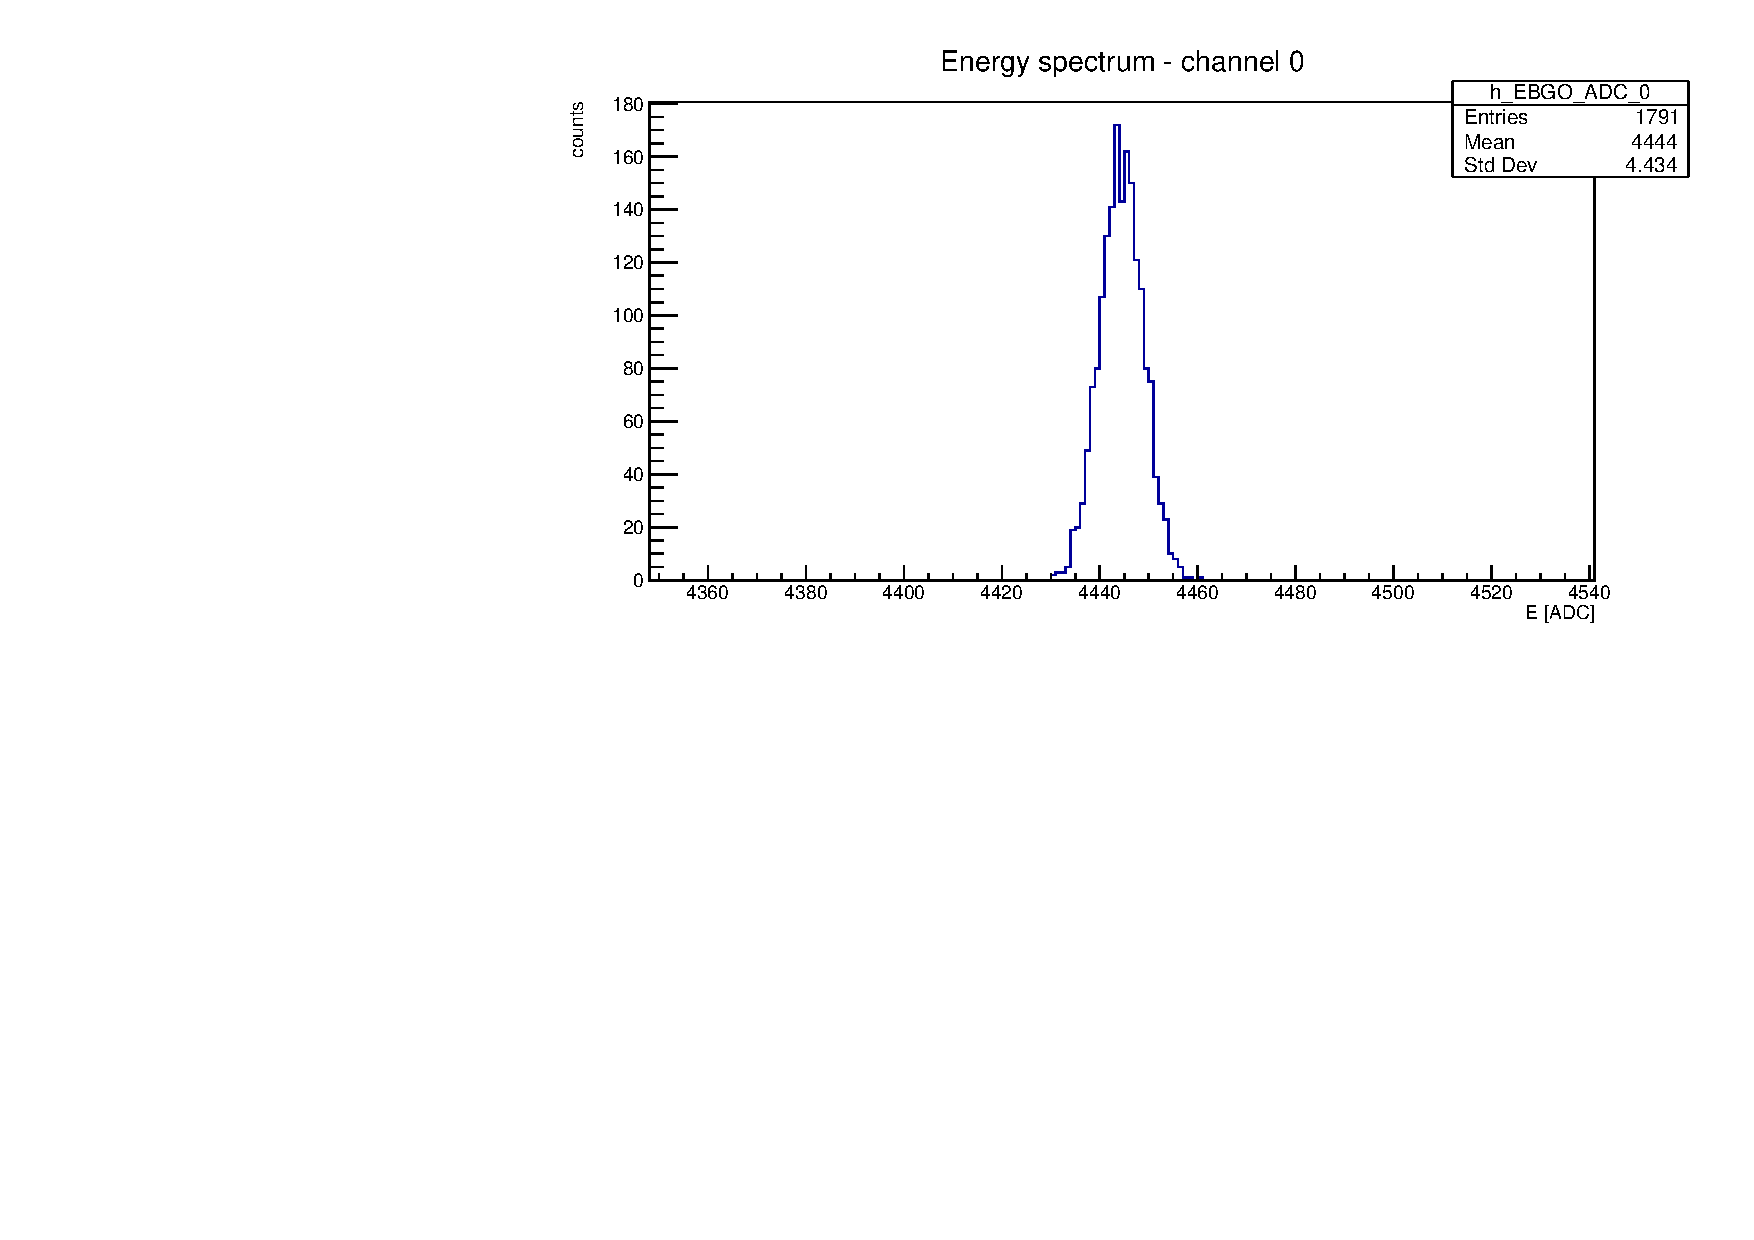
\includegraphics[width=\linewidth]{img/pulser.pdf} % Replace with your image path
		\end{minipage}
	\end{figure}
\end{frame}

\begin{frame}{Calcolo della calibrazione}
	\begin{itemize}
		\item La calibrazione viene effettuata sul file \texttt{run1775\_coinc.root}, con entrambe le sorgenti.
		\item \emph{Calibrare} uno scintillatore significa trovare il fattore di conversione da canali a energia.
		\item Per ogni spicchio del BGO si esegue un fit per trovare il valore dei picchi caratteristici e del picco somma in canali.
	\end{itemize}
\end{frame}

\begin{frame}{Calcolo della calibrazione}
	\begin{columns}
		\begin{column}{0.4\textwidth}
			\begin{itemize}
				\item<1-> I valori dei picchi vengono graficati contro quelli in energia caratteristici, noti.
				\item<3-> Si effettua dunque un fit lineare per i punti di ciascun istogramma.
				\item<4-> I coefficienti angolari di questi fit sono i fattori di conversione cercati.
			\end{itemize}
		\end{column}
		\begin{column}{0.5\textwidth}
			\begin{figure}
				\centering
				\only<2>{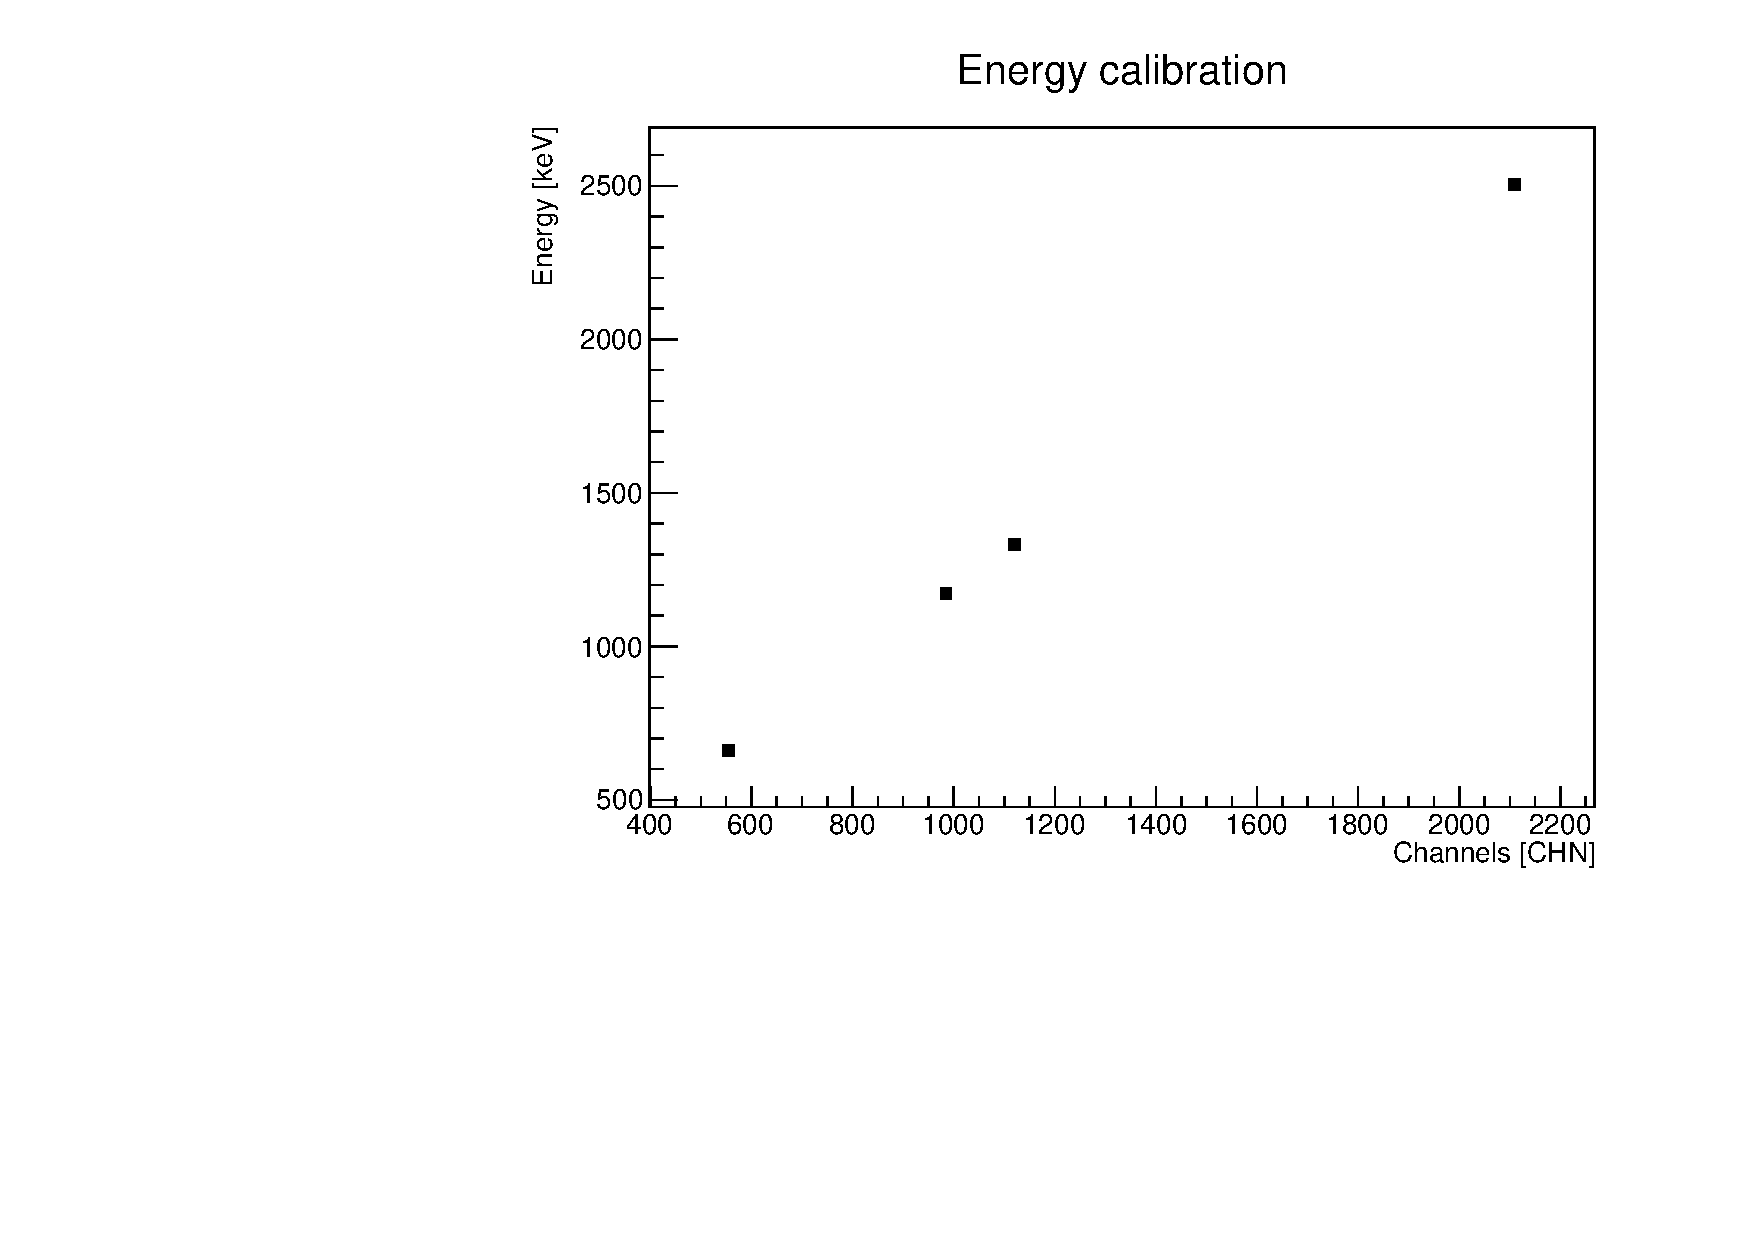
\includegraphics[width=0.9\textwidth]{img/plot0_empty.pdf}}
				\only<3->{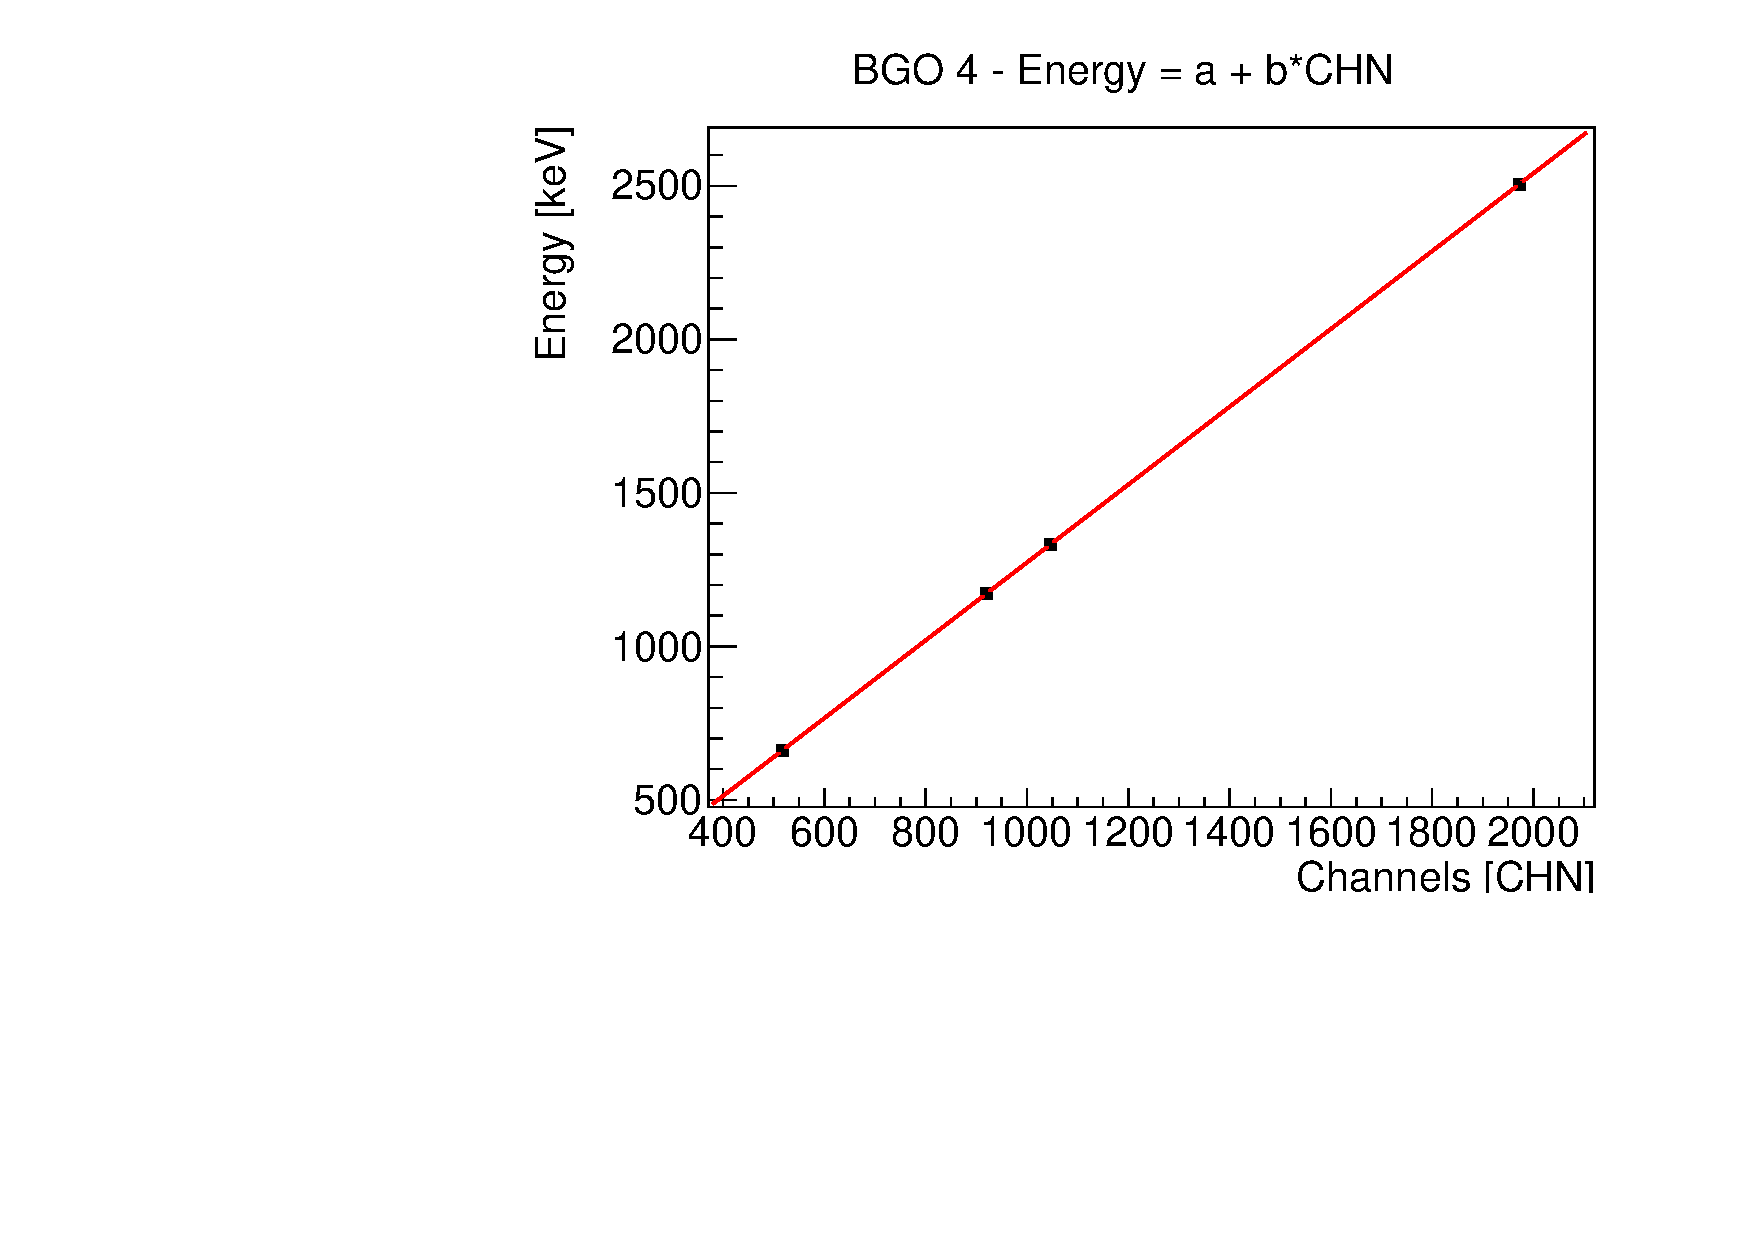
\includegraphics[width=0.9\textwidth]{img/plot0.pdf}}
				%TERZA GRAFICA PER FARE VEDERE I RISULTATI
			\end{figure}
		\end{column}
	\end{columns}
	
\end{frame}

\begin{frame}{Risultati del fit}
	\begin{table}[ht]
		\centering
		\resizebox{0.7\textwidth}{!}{
			\begin{tabular}{@{}cccc@{}}
				\toprule
				Canale & Conversione [keV/CHN] \\ \midrule
				CHN1 & 1.1863 \(\pm\) 0.0009 \\
				CHN2 & 1.1659 \(\pm\) 0.0013 \\
				CHN3 & 1.3550 \(\pm\) 0.0019 \\
				CHN4 & 1.2676 \(\pm\) 0.0006 \\
				CHN5 & 1.2574 \(\pm\) 0.0010 \\
				CHN6 & 1.1388 \(\pm\) 0.0014 \\
				\bottomrule
		\end{tabular}}
	\end{table}
\end{frame}

\begin{frame}{Residui}
	\begin{columns}
		\begin{column}{0.4\textwidth}
			\begin{itemize}
				\item<1-> I residui sono la differenza tra i valori in energia noti e quelli assunti dalla retta
				\item<2-> Sono una rappresentazione della bontà della calibrazione
				\item<3-> In generale una calibrazione è buona se i residui non superano la decina di keV
			\end{itemize}
		\end{column}
		\begin{column}{0.5\textwidth}
			\centering
			\only<2->{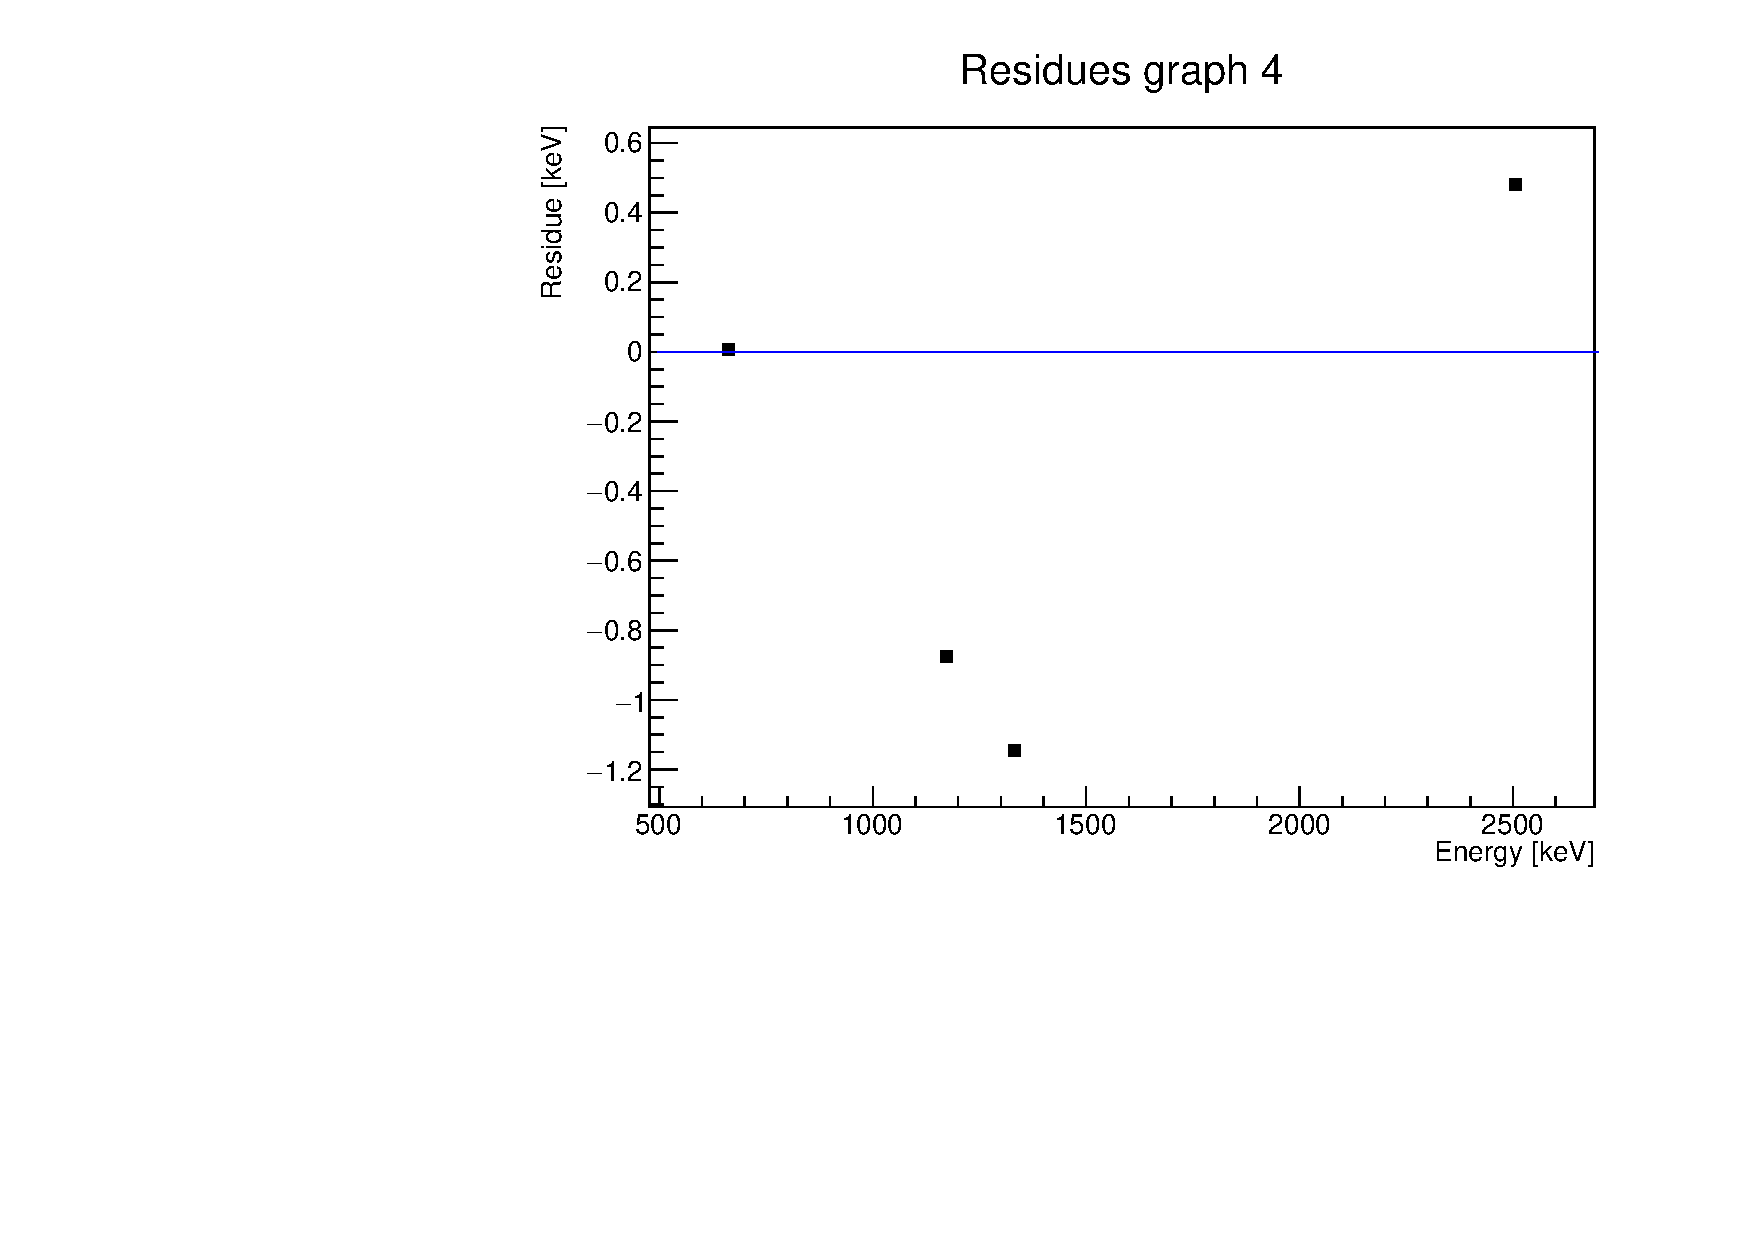
\includegraphics[width=0.9\textwidth]{img/residues0.pdf}}
		\end{column}
	\end{columns}
	
\end{frame}

\begin{frame}{Calcolo dell'efficienza}
	\begin{itemize}
		\item Per il calcolo dell'efficienza è necessario trovare il numero di conteggi nei picchi gaussiani. Si possono applicare due metodi diversi per trovarlo:
	\end{itemize}
	\hrule height 0.3mm \vspace{2mm}
	
	\begin{columns}
		\column{0.5\textwidth}
		\only<2->{\centering \emph{Trapezio} 
			\begin{itemize}
				\item Metodo geometrico
				\item Consiste nell'isolare la regione del picco e rimuoverne il fondo trapezoidale
				\item Adatto solo per il cesio: i due picchi del cobalto non sono sufficientemente risolti dallo strumento
		\end{itemize}}
		
		\column{0.5\textwidth}
		\only<3->{\centering \emph{Parametrico}
		\begin{itemize}
			\item Metodo che sfrutta i parametri del fit
			\item Il coefficiente di normalizzazione del picco gaussiano è il numero di conteggi nel picco
			\item Adatto per cesio e cobalto
	\end{itemize}}
	\end{columns}
			
\end{frame}
\begin{frame}{Metodo del trapezio}
	\centering
	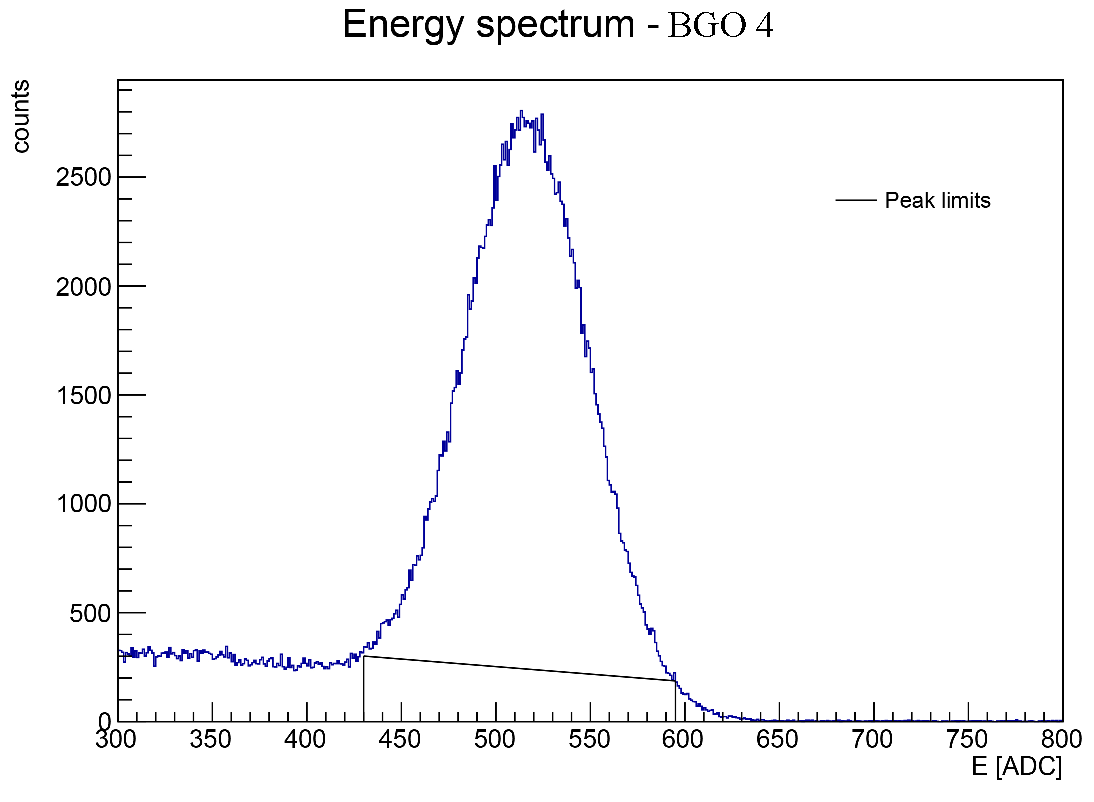
\includegraphics[width=0.9\textwidth]{img/trapezoid.pdf}
	\captionof{figure}{Visualizzazione del metodo del trapezio.}
\end{frame}
\begin{frame}{Attività e tempo vivo}
	contenuto...
\end{frame}
	
	\section{Conclusion}
	\begin{frame}{Conclusione}
		\begin{itemize}
			\item COME RAPPRESENTARE I RISULTATI???????????
		\end{itemize}
	\end{frame}
	
	\begin{frame}{Fine}
		\centering
		\textbf{Grazie per l'attenzione.}
	\end{frame}
	
\end{document}

